
% ---
% Simulação
% ---
\chapter{RESULTADOS PARCIAIS}
\label{cap:resultados_parciais}
% ---

Esse capítulo do trabalho apresenta o que foi desenvolvido no trabalho até o presente momento.

\section{Pesquisa exploratória sobre Revisões sistemática de literatura}
Inicialmente foi realizada uma pesquisa exploratória sobre a temática de Revisão Sistemática de Literatura, com o objetivo de entender mais sobre como funciona a metodologia e como deve ser aplicada. Nesse contexto, essa pesquisa procurou por guias que orientassem como aplicar a metodologia. Guias relacionadas com a área de computação foram explorados com maior atenção. 

Os trabalhos que mais se destacaram nesse sentido foram o \cite{kitchenham2007guidelines} e \cite{keele_guidelines_2007}, que apresentaram guias introdutórios mas bem completos tanto sobre a teoria, quanto sobre como aplicar a metodologia. No total foram encontrados quatorze trabalhos que davam algum tipo de orientação no processo de aplicação de Revisões Sistemáticas de Literatura relacionados com a área de computação. Inclusive dois deles o \cite{bai_conducting_2019} e o \cite{oosterwyk_synthesis_2019}, apresentam análises sobre os guias existentes.

\section{Ferramentas utilizadas e preparação do repositório do projeto}

Além do esforço realizado no entendimento sobre como realizar uma revisão sistemática de literatura, uma parte do tempo utilizado até o momento, o trabalho também tentou identificar quais ferramentas e técnicas poderiam ser utilizadas para conduzir uma revisão sistemática de literatura.

\subsection{Gerenciador de referências bibliográficas - Zotero}
Desde o início ficou claro que a utilização de uma ferramenta que pudesse realizar um gerenciamento das referências bibliográficas seria muito benéfica durante o desenvolvimento do trabalho. 

No total foram encontradas dezoito ferramentas que realizam esse tipo de trabalho. As que chamaram maior atenção foram RefWorks, a EndNote a Mendeley e a Zotero. 

De uma maneira geral, as quatro ferramentas analisadas possuem uma versão desktop do software, mas que permitem armazenamento dos dados em nuvem. É possível também ter acesso aos dados através de uma aplicação web disponibilizada pelos seus fabricantes.

As ferramentas também possuem recursos que possibilitam exportar as referências bibliográficas como bibliografias para editores de texto como o Microsoft Word, e templates que definem o padrão dessa bibliografia e da forma como a citação desse trabalho aparece no texto.

Normalmente também possuem plugins que podem ser instalados nos navegadores web, permitindo importar links resultantes de buscas em repositórios de artigo, para as suas bases e catálogos de referências bibliográficas.

Algumas delas possuem integração com repositórios de artigos científicos, que permitem realizar as buscas diretamente nesses repositórios.

A ferramenta de gerenciamento de referências bibliográficas escolhida para esse trabalho foi a Zotero. Os principais motivos que levaram a adoção dessa ferramenta foram: 

\begin{enumerate}
    \item Por ser um software livre;
    \item Por ser uma ferramenta madura, que está em desenvolvimento desde 2006;
    \item Por ser gratuita;
    \item e por possuir funcionalidades como:
        \begin{enumerate}
            \item Importação e exportação de referência bibliográficas;
            \item A recuperação de documentos a partir de referência importada; 
            \item Por ser multi-plataforma, disponível para diversos tipos de sistemas operacionais;
            \item Ter um serviço público de nuvem, que permite criar grupos e dar acesso de leitura e escrita aos catálogos criados;
        \end{enumerate}
\end{enumerate}

\subsection{LaTeX - Overleaf}

O LaTeX foi escolhido como ferramenta de edição para a dissertação. O texto produzido para da qualificação também já foi desenvolvido em LaTeX.

A escolha do LaTeX se deu por entender que a saída do gerenciador de referência bibliográfica, pode ser realizada em Padrão BibTex. que é o formato de referência bibliográfica padrão do LaTeX. 

Além do gosto pessoal da utilização do LaTeX, outro ponto interessante na escolha desse formato de texto, é que uma vez superada a curva de aprendizado da utilização da ferramenta, a organização estrutural do trabalho fica muito independente da sua formatação. 

A consistência na utilização das citações também é um fator que merece destaque. O seu funcionamento impede que existam citações sem a devida entrada na seção de referências bibliográficas, bem como não adicionará a essa seção do texto, uma referência que não tiver sido explicitamente citada.

A apesar de ter sido configurado um ambiente local com controle de versão do texto para o desenvolvimento do trabalho, optou-se por trabalhar no editor da Overleaf, que é um serviço de nuvem que permite edição de textos em LaTeX, e que poder ser feito de forma colaborativa, o que facilitou o trabalho de revisão da orientadora.

\subsection{Repositório do projeto - Github}

O GitHub foi escolhido como repositório do projeto. Todos os artefatos gerados durante o trabalho serão armazenados no seguinte repositório \cite{repositorioGithub}, e lá e estarão disponíveis para consulta por qualquer pessoa interessada no trabalho. 

Também será criado um identificador único para esse repositório, através de um DOI, disponibilizado pela ferramenta Zenodo. A ideia é tentar tornar o estudo mais acessível e reprodutível.  

\section{Pesquisa exploratória de Revisões sistemática de literatura relacionadas com programação concorrente}

Foi realizada uma pesquisa exploratória das revisões sistemática de literatura relacionadas com técnicas de  validação e verificação de programas concorrentes, que é o objeto de estudo desse trabalho. Nesse momento o escopo da pesquisa não se limitou apenas aos programas que se apoiam em troca de mensagem, incluindo também a programação que utiliza memória compartilhada para a comunicação entre os processos.

Os detalhes dessas pesquisa foi utilizada como base para o capítulo \ref{cap:trabalhos_relacionados}, dos trabalhos relacionados.

\section{Teste de execução de revisão sistemática no repositório do IEEE Xplore}

Durante o desenvolvimento do estudo foi realizado um testes do processo de pesquisa normalmente utilizada na revisão sistemática de literatura. A ideia desse teste era entender os seguintes pontos:

\begin{enumerate}
    \item Testar qual a dinâmica de uma pesquisa feita de forma sistemática, utilizando uma string de busca pré-definida;
    \item Entender o volume de artigos realizados para uma string de busca relacionada ao assunto que será pesquisado; 
    \item Entender a dinâmica de uma string de busca mais específica e de uma string de busca mais genérica;
    \item Ter uma ideia do tempo que seria necessário para selecionar os estudos primários em um repositório;
\end{enumerate}

\subsection{Testes com a string de busca}

A string utilizada nesses testes foi a seguinte:

\begin{verbatim}
(
    ("title + abstract":message passing)  
    AND(
          "title + abstract":test*
          OR "title + abstract":check*
          OR "title + abstract":validat* 
          OR "title + abstract":verif* 
    ) 
)
\end{verbatim}

Inicialmente essa string foi disparada em alguns dos repositórios listados na seção \ref{subsec:repositoriosPesquisa}, e essa experiência gerou algumas descobertas:

\begin{enumerate}
    \item Constatou-se que nas pesquisas tanto as expressões booleanas quanto os metadados disponíveis para pesquisa, variam um pouco entre os diversos repositórios, e com isso, as strings de busca precisam ser adaptadas para manter o mesmo sentido durante a execução das buscas;
    \item Os artigos utilizando a string de busca escolhida, trouxe a maior parte dos resultados com publicação mais antigas que dez anos;
    \item O repositório do IEEE  Xplore \cite{repositorioIEEE} foi o que retornou o maior número de resultados dentre os repositórios testados; 
\end{enumerate}

\subsection{Resultado da pesquisa no IEEE Xplore}

Por ter o maior número de resultados na busca, o repositório IEEE Xplorer foi escolhido para aprofundar os testes com a dinâmica da etapa de pesquisa da revisão sistemática de literatura.

Durante a execução dos testes, percebeu-se que a string utilizada no repositório do IEEE Xplorer retornou como resultado quatro mil cento e setenta e três documentos. Com isso percebeu-se que o a string de busca utilizada era muito genérica, e que provavelmente precisaria ser revisada durante a fase de pesquisa do trabalho.

A Figura\ref{fig:rsltest} apresenta o processo que foi utilizado durante a pesquisa exploratória de teste.

\begin{figure}[h!]
\centering
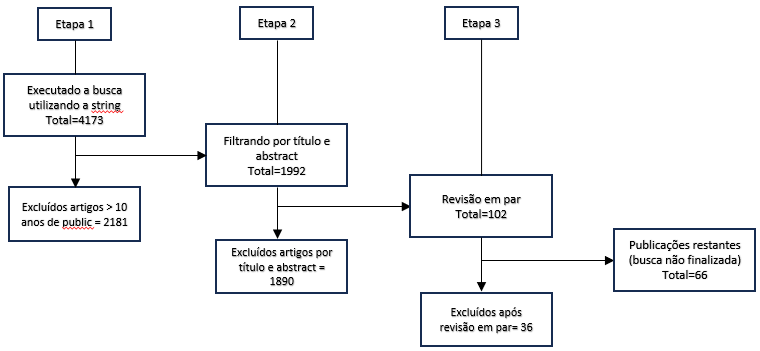
\includegraphics[width=1\textwidth]{img/rslteste.png}
\caption{Procedimento de seleção de estudos do teste.}
\label{fig:rsltest}
\end{figure}

Apesar do último filtro de artigos não ter sido realizado durante a fase de teste, entendeu-se que para o proposito de testes, esse esforço era o suficiente. As experiências obtidas através desse teste conseguiu esclarecer os principais pontos elencados no início desse seção além de mais algumas respostas:

 \begin{enumerate}
     \item Foi possível entender um pouco sobre a forma e sutiliza da execução das pesquisas entre diferentes repositórios de busca;
     \item Ter uma noção do sobre a quantidade de documentos que precisarão ser filtrados durante o processo de seleção dos estudos primários;
     \item Ter também uma ideia doo tempo necessário para realizar esse seleção;
     \item Foi possível também perceber que a string de busca muito genéria traz um resultado com muitos documentos, e que esse string precisaria ser refinada;
     \item Foi possível refinar e desenhar um melhor processo para a execução da pesquisa;
 \end{enumerate}